\documentclass[]{article}

\usepackage[left=2.00cm, right=2.00cm, top=2.00cm, bottom=2.00cm]{geometry}
\usepackage[spanish,es-noshorthands]{babel}
\usepackage[utf8]{inputenc} % para tildes y ñ
\usepackage{graphicx} % para las figuras
\usepackage{xcolor}
\usepackage{listings} % para el código fuente en c++

\lstdefinestyle{customc}{
  belowcaptionskip=1\baselineskip,
  breaklines=true,
  frame=single,
  xleftmargin=\parindent,
  language=C++,
  showstringspaces=false,
  basicstyle=\footnotesize\ttfamily,
  keywordstyle=\bfseries\color{green!40!black},
  commentstyle=\itshape\color{gray!40!gray},
  identifierstyle=\color{black},
  stringstyle=\color{orange},
}
\lstset{style=customc}


%opening
\title{Práctica 1. Algoritmos devoradores}
\author{Lucía Atienza Olmo \\ % mantenga las dos barras al final de la línea y este comentario
lucia.atienzaolmo@alum.uca.es \\ % mantenga las dos barras al final de la línea y este comentario
Teléfono: 646767043 \\ % mantenga las dos barras al final de la linea y este comentario
NIF: 32089267n  \\ % mantenga las dos barras al final de la línea y este comentario
}


\begin{document}

\maketitle

%\begin{abstract}
%\end{abstract}

% Ejemplo de ecuación a trozos
%
%$f(i,j)=\left\{ 
%  \begin{array}{lcr}
%      i + j & si & i < j \\ % caso 1
%      i + 7 & si & i = 1 \\ % caso 2
%      2 & si & i \geq j     % caso 3
%  \end{array}
%\right.$

\begin{enumerate}
\item Describa a continuación la función diseñada para otorgar un determinado valor a cada una de las celdas del terreno de batalla para el caso del centro de extracción de minerales. 

$$ f(rango, coste, dispersion, danno)=2 * (rango - danno - 2*dispersion) + 1.7 * (danno - 0.2*coste) $$


\item Diseñe una función de factibilidad explicita y descríbala a continuación.

\begin{lstlisting}
void DEF_LIB_EXPORTED calculatePath(AStarNode* originNode, AStarNode* targetNode
                   , int cellsWidth, int cellsHeight, float mapWidth, float mapHeight
                   , float** additionalCost, std::list<Vector3> &path) 
{
    bool found = false;
    std::vector<AStarNode*> closed, opened;
    AStarNode* cur = originNode;
    int x, y;
    positionToCell((cur)->position, x, y, cellsWidth, cellsHeight);
    cur->H = estimatedDistance(originNode, targetNode, x, y, additionalCost);
    cur->G = 0; 
    cur->F = cur->G + cur->H;
    opened.push_back(cur);
    std::make_heap(opened.begin(), opened.end(), min);
    while(!found && opened.size() > 0) //mientras no se encuentre solucion y queden nodos disponibles
    {
        std::pop_heap(opened.begin(), opened.end(), min);
        cur = opened.back();
        opened.pop_back(); 
        closed.push_back(cur);
        if(iguales(cur, targetNode))
            found = true;
        else
        {
            List<AStarNode*>::iterator j; 
            for(j = cur->adjacents.begin(); j != cur->adjacents.end(); ++j) 
            {
                if(std::find_if(closed.begin(), closed.end(), isEqualTo(*j)) == std::end(closed)) //no se encuentra en cerrados
                {
                    if(std::find_if(opened.begin(), opened.end(), isEqualTo(*j)) == std::end(opened)) //no se encuentra en abiertos
                    {
                        (*j)->parent = cur;
                        (*j)->G = cur->G + _distance(cur->position, (*j)->position);
                        int row,col;
                        positionToCell((*j)->position, row, col, cellsWidth, cellsHeight);
                        (*j)->H = estimatedDistance(*j, targetNode, row, col, additionalCost);
                        (*j)->F = (*j)->G + (*j)->H;
                        opened.push_back(*j);
                        std::push_heap(opened.begin(), opened.end(), min);
                    }
                    else //se ha encontrado en abiertos
                    {
                        float d = _distance(cur->position, (*j)->position);
                        if((*j)->G > cur->G + d)
                        {
                            (*j)->parent = cur;
                            (*j)->G = cur->G + d;
                            (*j)->F = (*j)->G + (*j)->H;
                            std::sort_heap(opened.begin(), opened.end(), min);
                        }
                    }
                }
            }
        }
    }
    if(found) //si hemos encontrado solucion, recuperamos camino
    {
        cur = targetNode;
        path.push_front(targetNode->position);
		while(cur->parent != originNode)
		{
			cur = cur->parent;
			path.push_front(cur->position);
		}
    }
}
\end{lstlisting}

\item A partir de las funciones definidas en los ejercicios anteriores diseñe un algoritmo voraz que resuelva el problema para el caso del centro de extracción de minerales. Incluya a continuación el código fuente relevante. 

\begin{lstlisting}
void DEF_LIB_EXPORTED placeDefenses(bool** freeCells, int nCellsWidth, int nCellsHeight, float mapWidth, float mapHeight,
             std::list<Object*> obstacles, std::list<Defense*> defenses) 
{
    float cellWidth = mapWidth / nCellsWidth;
    float cellHeight = mapHeight / nCellsHeight; 
    std::vector<std::vector<celda> > mapa(nCellsHeight, std::vector<celda>(nCellsWidth));
    std::list<Defense*> copiaDefensas = defenses;
    std::list<Defense*>::iterator centroExtraccion = defenses.begin();
    std::list<celda> listaCeldas;
    rellenaMapa(mapa, obstacles, nCellsWidth, nCellsHeight, mapWidth, mapHeight);
    rellenaLista(mapa, listaCeldas, nCellsWidth, nCellsHeight);
    bool colocado = false;
    while(!listaCeldas.empty() && !colocado)
    {
        celda mejorPosicion = extraeCelda(listaCeldas);
        if(factible(mejorPosicion.row, mejorPosicion.col, nCellsWidth, nCellsHeight, mapWidth, mapHeight, obstacles, defenses, *centroExtraccion))
        {
            (*centroExtraccion)->position = cellToPosition(mejorPosicion.row, mejorPosicion.col, cellWidth, cellHeight);
            colocado = true;
        }
    }
}
\end{lstlisting}

\item Comente las características que lo identifican como perteneciente al esquema de los algoritmos voraces. 

\begin{lstlisting}
//funcion para comprobar si un vector esta ordenado o no
bool compruebaOrdenado(std::vector<int> v)
{
    for(int i = 0; i < v.size()-1; i++)
    {
        if(v[i] > v[i+1])
            return false;
    }
    return true;
}

int main()
{
    std::vector<int> v;
    std::cout << "[Ordenacion rapida] Para un vector de 5 elementos, 120 combinaciones posibles" << std::endl; 
    for(int i = 0; i < 5; i++)
        v.push_back(i);
    int ordenadas = 0;
    do{
        std::vector<int> aux = v;
        ordenacion_rapida(aux, 0, aux.size());
        if(compruebaOrdenado(aux))
            ordenadas++;
    }while(std::next_permutation(v.begin(), v.end()));
    std::cout << "Numero de permutaciones ordenadas: " << ordenadas << std::endl; 
}
\end{lstlisting}

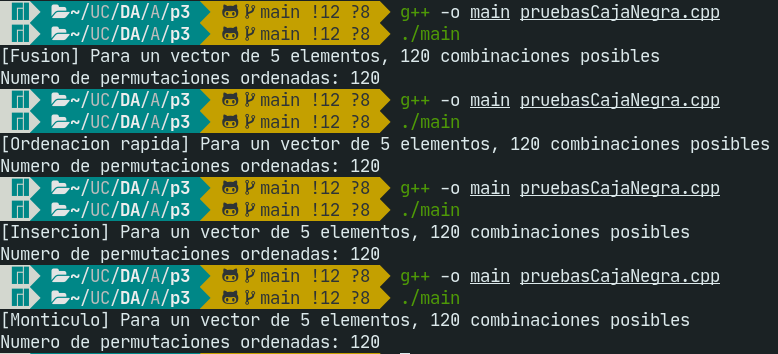
\includegraphics[scale=0.6]{DA.png} 

\item Describa a continuación la función diseñada para otorgar un determinado valor a cada una de las celdas del terreno de batalla para el caso del resto de defensas. Suponga que el valor otorgado a una celda no puede verse afectado por la colocación de una de estas defensas en el campo de batalla. Dicho de otra forma, no es posible modificar el valor otorgado a una celda una vez que se haya colocado una de estas defensas. Evidentemente, el valor de una celda sí que puede verse afectado por la ubicación del centro de extracción de minerales.

A cada celda se le ha dado el valor de la distancia entre dicha celda y el centro de extracción de minerales. A este valor se 
le ha aplicado la misma ponderaci\'on descrita en el primer ejercicio de los valores de las posiciones del mapa (cuanto m\'as 
centradas est\'en mayores valores tienen).

\item A partir de las funciones definidas en los ejercicios anteriores diseñe un algoritmo voraz que resuelva el problema global. Este algoritmo puede estar formado por uno o dos algoritmos voraces independientes, ejecutados uno a continuación del otro. Incluya a continuación el código fuente relevante que no haya incluido ya como respuesta al ejercicio 3. 

\begin{lstlisting}
    cronometro SO;
    long int r1 = 0;
    const double e_abs = 0.01, e_rel = 0.001;
    SO.activar();
    do {
        placeDefenses_SO(freeCells, nCellsWidth, nCellsHeight, mapWidth, mapHeight, obstacles, defenses);
	++r1;
    } while(SO.tiempo() < e_abs / e_rel + e_abs);
    SO.parar();

    cronometro OR;
    long int r2 = 0;
    OR.activar();
    do {
        placeDefenses_OR(freeCells, nCellsWidth, nCellsHeight, mapWidth, mapHeight, obstacles, defenses);
	++r2;
    } while(OR.tiempo() < e_abs / e_rel + e_abs);
    OR.parar();

    cronometro F;
    long int r3 = 0;
    F.activar();
    do {
        placeDefenses_F(freeCells, nCellsWidth, nCellsHeight, mapWidth, mapHeight, obstacles, defenses);
	    ++r3;
    } while(F.tiempo() < e_abs / e_rel + e_abs);
    F.parar();
    
    cronometro M;
    long int r4 = 0;
    M.activar();
    do {
        placeDefenses_M(freeCells, nCellsWidth, nCellsHeight, mapWidth, mapHeight, obstacles, defenses);
	    ++r4;
    } while(M.tiempo() < e_abs / e_rel + e_abs);
    M.parar();
    std::cout << (nCellsWidth * nCellsHeight) << "\t" << SO.tiempo() / r1 << "\t" << F.tiempo() / r3 << "\t" << OR.tiempo() / r2 << "\t" << M.tiempo() / r4 << std::endl;
\end{lstlisting}
\begin{center}
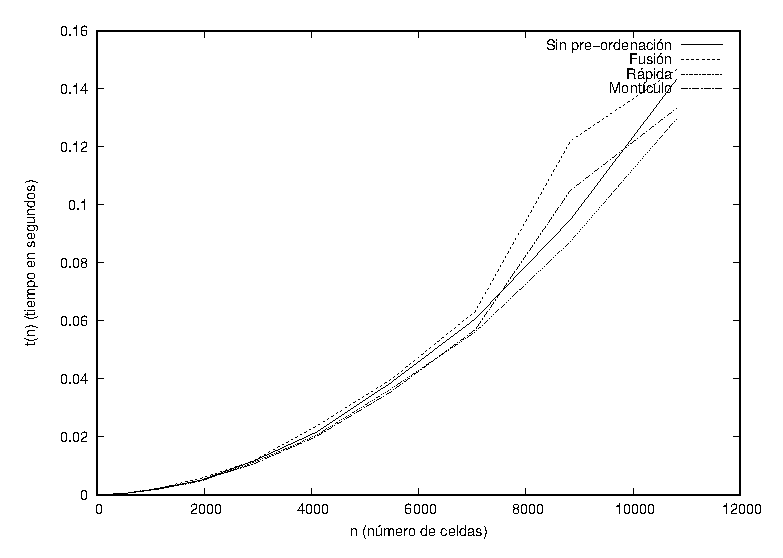
\includegraphics[scale=0.9]{graphic.eps} 
\end{center}

\end{enumerate}

Todo el material incluido en esta memoria y en los ficheros asociados es de mi autoría o ha sido facilitado por los profesores de la asignatura. Haciendo entrega de este documento confirmo que he leído la normativa de la asignatura, incluido el punto que respecta al uso de material no original.

\end{document}
